\documentclass{book}
\usepackage{graphicx}                              %for PNG images (pdflatex)
\usepackage[linkbordercolor={1.0 1.0 0.0}]{hyperref} %for \url tag
\usepackage{color}                                 %for defining custom colors
\usepackage{framed}                                %for shaded and framed paragraphs
\usepackage{textcomp}                              %for various symbols, e.g. Registered Mark
\usepackage{geometry}                              %for defining page size
\usepackage{longtable}                             %for breaking tables
%
\geometry{verbose,a4paper,tmargin=2.5cm,bmargin=2.5cm,lmargin=2.5cm,rmargin=2cm}
\hypersetup{
  pdfauthor = {Zsombor Nagy},
  pdftitle = {Documentation of the ARC storage system},
  pdfsubject = {Paper subject},
  pdfkeywords = {Paper,keyword,comma-separated},
  pdfcreator = {PDFLaTeX with hyperref package},
  pdfproducer = {PDFLaTeX}
}
%
\bibliographystyle{IEEEtran}                       %a nice bibliography style
%
\def\efill{\hfill\nopagebreak}%
\hyphenation{Nordu-Grid}
\setlength{\parindent}{0cm}
\setlength{\FrameRule}{1pt}
\setlength{\FrameSep}{8pt}
\addtolength{\parskip}{5pt}
\renewcommand{\thefootnote}{\fnsymbol{footnote}}
\renewcommand{\arraystretch}{1.3}
\newcommand{\dothis}{\colorbox{shadecolor}}
\newcommand{\ngdl}{\url{http://ftp.nordugrid.org/download}~}
\definecolor{shadecolor}{rgb}{1,1,0.6}
\definecolor{salmon}{rgb}{1,0.9,1}
\definecolor{bordeaux}{rgb}{0.75,0.,0.}
\definecolor{cyan}{rgb}{0,1,1}
%
%----- DON'T CHANGE HEADER MATTER
\hyphenation{preserve-Original}
\begin{document}
\def\today{\number\day/\number\month/\number\year}

\begin{titlepage}

\begin{tabular}{rl}
\resizebox*{3cm}{!}{
\includegraphics{ng-logo.png}}
&\parbox[b]{2cm}{\textbf \it {\hspace*{-1.5cm}NORDUGRID\vspace*{0.5cm}}}
\end{tabular}

\hrulefill

%-------- Change this to NORDUGRID-XXXXXXX-NN

{\raggedleft NORDUGRID-TECH-17\par}

{\raggedleft \today\par}

\vspace*{2cm}

%%%%---- The title ----
{\centering \textsc{\Large Documentation of the ARC storage system}\Large \par}
\vspace*{0.5cm}
    
%%%%---- A subtitle, if necessary ----
{\centering \textit{\large First prototype status and plans}\large \par}
    
\vspace*{1.5cm}
%%%%---- A list of authors ----
    {\centering \large Zsombor Nagy\footnote{zsombor@niif.hu} \large \par}
    {\centering \large Jon Nilsen\footnote{j.k.nilsen@usit.uio.no} \large \par}
    {\centering \large Salman Zubair Toor \footnote{salman.toor@it.uu.se} \large \par}
\end{titlepage}

\tableofcontents                          %Comment if use article style
\newpage

\renewcommand{\thefootnote}{\arabic{footnote}}


\chapter{Design Overview} % (fold)
\label{cha:overview}


The ARC storage system is a distributed system for storing replicated \emph{file}s on several file storage nodes and manage them in a global namespace.  The files can be grouped into \emph{collection}s (a concept very similar to directories in the common file systems), and a collection can contain sub-collections and sub-sub-collections in any depth. There is a dedicated \emph{root collection} to gather all collections to the global namespace. This hierarchy of collections and files can be referenced using \emph{Logical Name}s (\emph{LN}s). The users can use this global namespace as they were using a local filesystem. Files can be transfered by multiple transfer protocols, and the client side tools hide this from the user. The replicas of the files are stored on different storage nodes. A storage node here is a network-accessible computer having storage space to share, and a storage element service running (e.g.~HTTP(S), FTP(S), GridFTP, ByteIO\footnote{OGSA ByteIO Working Group (BYTEIO-WG), \url{https://forge.gridforum.org/projects/byteio-wg/}}, etc.). For each storage node one of the services of the ARC storage system is needed to manage it and to integrate it into the system. There is a way on the client side to access third-party storage solutions through the namespace of the ARC storage system. The main services of the storage system are the following (see Figure~\ref{fig:services}):
\begin{itemize}
    \item the \textbf{A-Hash} service, which is a replicated database which is used by the Librarian to store metadata;
    \item the \textbf{Librarian} service, which handles the metadata and hierarchy of collections and files, the location of replicas, and health data of the Shepherd services, using the A-Hash as database;
    \item the \textbf{Bartender} service, which provides a high-level interface for the users and for other services;
    \item the \textbf{Shepherd} service, which manages storage element services, and provides a simple interface for storing files on storage nodes.
\end{itemize}

\begin{figure}[ht]
\centering{{\scalebox{0.9}{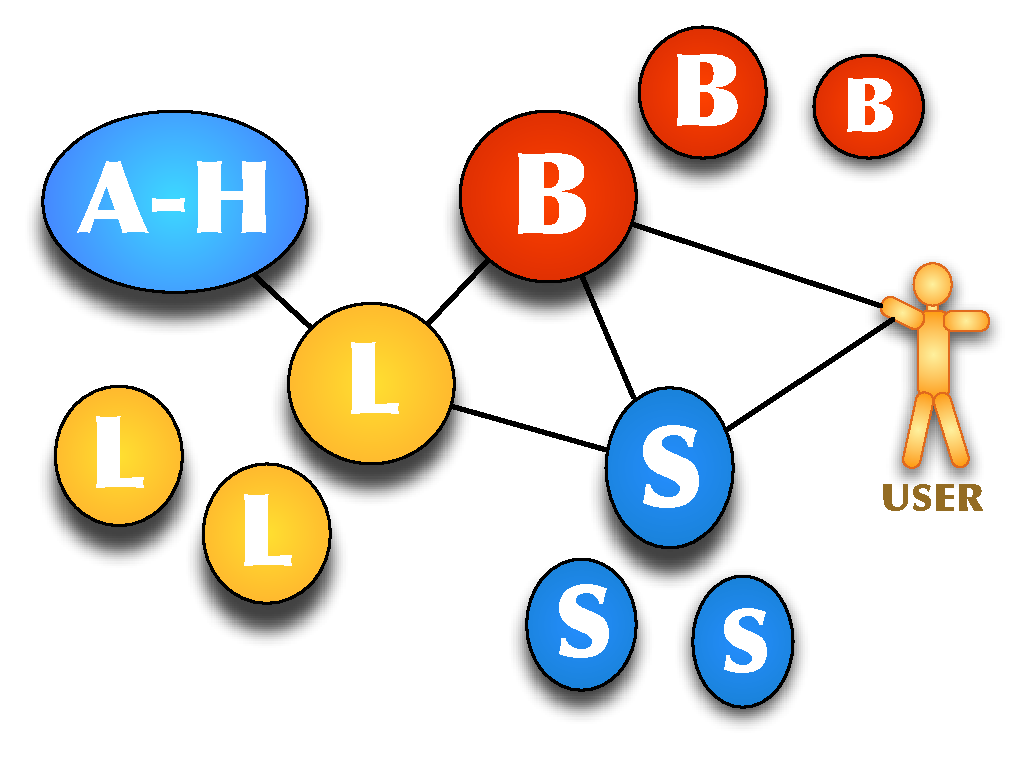
\includegraphics{arc-storage-services.pdf}}}
\caption{\label{fig:services}The components of the ARC storage: the \textbf{A-H}ash service, the \textbf{L}ibrarian service, the \textbf{B}artender service and the \textbf{S}hepherd service.}}
\end{figure}

\section{Files and collections} % (fold)
\label{sec:files_and_collections}

The storage system is capable of storing files which can be grouped in collections and sub-collections, etc.
Every file and collection has a unique ID in the sysem called the \emph{GUID}. Compared to the well-known structure of local file systems, these GUIDs are very similar to the concept of \emph{inode}s. And as a directory on a local filesystem is basically just a list of name and inode pairs, a collection on the ARC storage is just a list of name and GUID pairs. There is a dedicated collection which is the \emph{root collection}. This makes the namespace of the ARC storage system a hierarchical namespace where you can start at the root collection, and go to sub-collections and sub-sub-collections to get to a file. This path is called the \emph{Logical Name} (LN). For example if there is a sub-collection called \verb!saturn! in the root collection, and there is a file called \verb!rings! in this sub-collection, then the LN of this file is \verb!/saturn/rings!.

Besides the Logical Names we can refer to a file or collection by simply its GUID, or we can use GUIDs and Logical Names together, as seen on Figure~\ref{fig:namespace}.

The full syntax of Logical Names is \verb#/[path]# or \verb#<GUID>[/<path>]# where [...] indicates optional parts.

\begin{figure}[ht]
\centering{{\scalebox{0.7}{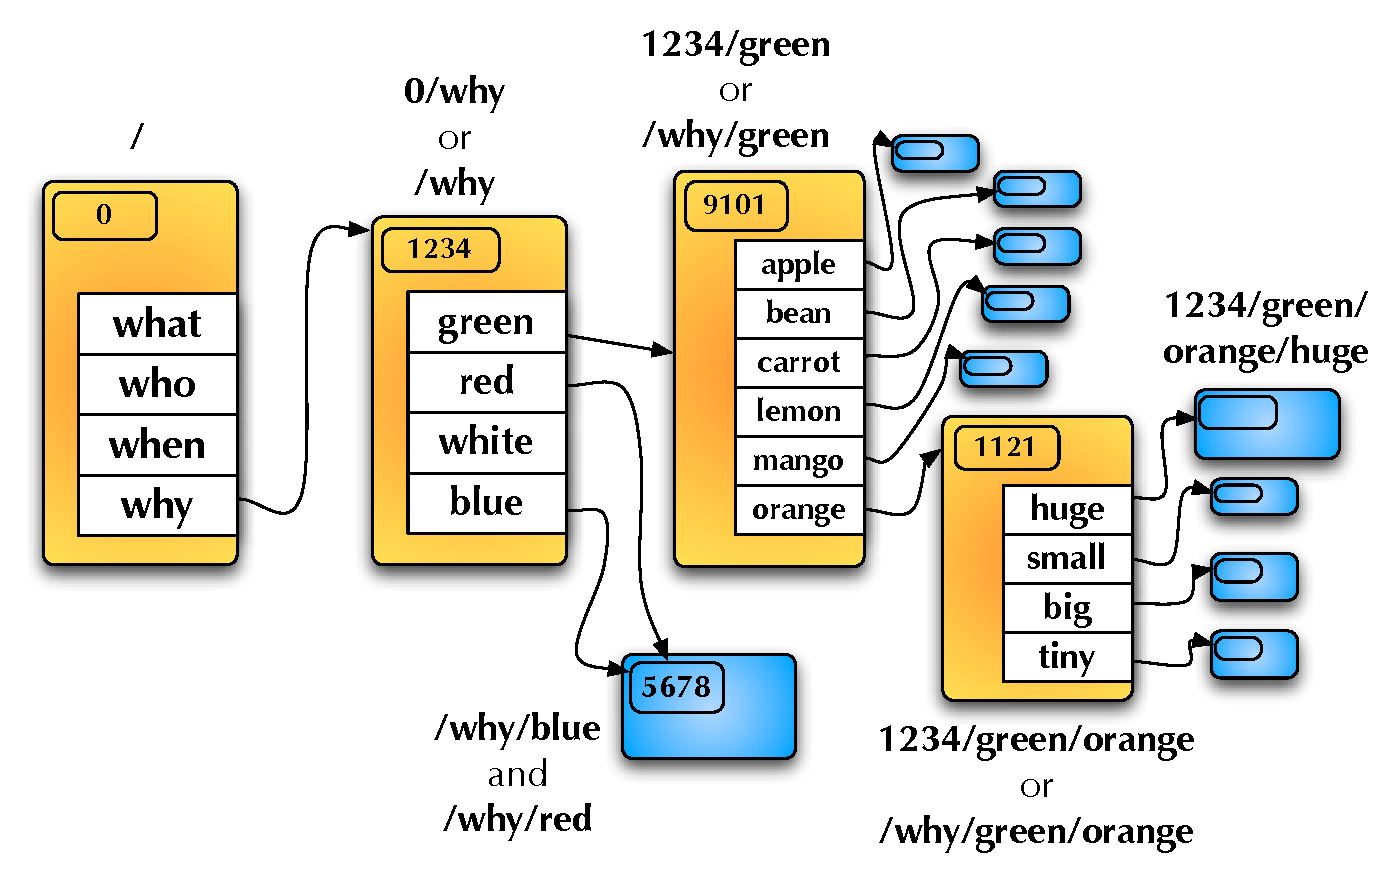
\includegraphics{arc-storage-namespace.pdf}}}
\caption{\label{fig:namespace}Example of the hierarchy of the global namespace} }
\end{figure}

Example on Figure~\ref{fig:namespace}: if we have a collection with GUID \verb#1234#, and there is a collection called \verb#green# in it, and in \verb#green# there is another collection called \verb#orange#, and in \verb#orange# there is a file called \verb#huge#, then we can refer to this file with the Logical Name \verb#1234/green/orange/huge#, which means that from the collection called \verb!1234! we have to follow along the path: \verb!green!, \verb!orange!, \verb!huge!.

There is a dedicated root collection (which has the GUID \verb#0#), and if a LN starts with no GUID prefix, it is implicitly prefixed with the GUID of this well-known root collection, e.g.~\verb#/why/blue# means \verb#0/why/blue#. If a user wants to find the file called \verb#/why/blue#, the system knows where to start the search: the GUID of the root collection. The root collection knows the GUID of \verb#why#, and the (sub-)collection \verb#why# knows the GUID of \verb#blue#. If the GUID of this file is \verb#5678#, and somebody makes another entry in collection \verb#/why# (= \verb#0/why#) with name \verb#red# and GUID \verb#5678#, then the \verb#/why/red# LN points to the same file as \verb#/why/blue#, which concept is very similar to a hardlink in a regular local file system.

% section files_and_collections (end)

\section{Storage nodes and replicas} % (fold)
\label{sec:storage_nodes_and_replicas}

The collections in the ARC storage are logical entities, the content of a collection is stored as metadata of the collection, which means the a collection actually has no physical data. A file however has both metadata and real physicial data (the actual bytes of the file). The metadata of a file is stored in the same database where the collections are stored, but the physical data of a file is stored on storage nodes as multiple replicated copies.

A storage node consists of two things: a storage element service which is capable of storing and serving files through a specific protocol (e.g. a web server, an FTP server, a GridFTP server, etc.) and a Shepherd service which provides a simple interface to access the storage node, and which can initiate and manage file transfers through the storage element service. The Shepherd has different backends for the supported storage element services which made it possible the communicate with them.

So we have logical files, which are part of the hierarchical namespace and have a GUID and other metadata, and a logical file has one or more physical replicas. The physical replicas stored on seperate storage nodes. In order to connect the logical file to its replicas, we need to have some pointers. Each storage node has a URL and each replica has a unique ID within the storage node called \emph{referenceID}, the URL and the referenceID together is called a \emph{Location}, a Location unambiguously points to one specific replica. So to connect the logical files to the physical ones, each logical file has a list of Locations.

The user can specify for each file how many replicas are needed. The ARC storage system periodically checks the number of replicas, and automatically creates new replicas if there are fewer then needed, and removes replicas if there are more. 

The different replicas of a file could be in different states, e.g. the replica could be valid and alive or just in the process of creation or it could be corrupt or a whole storage node could be offline. This state is always stored as metadata next to the Location of the given replica. For each file there is a checksum calculated, and this checksum is used to detect if a replica gets corrupted. If a storage node (more precisely: the Shepherd service on the storage node) detects that a file is invalid, it reports this so the metadata will be in sync with the real state. And the storage nodes sends heartbeat messages periodically, and if a storage node goes offline, the missing heartbeat triggers the modification of metadata as well. 

% section storage_nodes_and_replicas (end)

\section{The A-Hash} % (fold)
\label{sec:the_a_hash}

The A-Hash is a replicated metadata store, which is capable of consistently storing `objects' where an object contains key-value pairs organized in sections. All metadata about files and collections are stored in the A-Hash, and some other information (e.g. about A-Hash replication, about Shepherd services, etc.) is stored in it as well. The A-Hash itself does not interpret the data, it basically just stores tuples of strings.

% section the_a_hash (end)

\section{The Librarians} % (fold)
\label{sec:the_librarians}

The Librarian is capable of managing the hierarchy and metadata of files and collections, and health information of the Shepherd services. It can traverse Logical Names and return the corresponding metadata. It can receive heartbeat messages from Shepherd services, and it automatically modify the states of files if needed. The Librarian itself is a stateless service, it uses the A-Hash to actually store and retrieve the metadata, that’s why there could be any number of independent Librarian services (all using the same A-Hashes) which provides high-availability and load-balancing.

% section the_librarians (end)

\section{The Bartenders} % (fold)
\label{sec:the_bartenders}

The Bartender service provides a high-level interface for the storage system to the clients. Every interaction between a client and the ARC storage system begins with a request to a Bartender. You can create and remove collections, create, get and remove files, move files and collections within the namespace using Logical Names. The Bartender authorizes users and force access policies of files and collections. It communicates with the Librarian and Shepherd services to accomplish the client’s requests. The actual file data does not go through the Bartender; file transfers are directly performed between the storage nodes and the clients. There could be any number of independent Bartender services in the system which provides high-availability and load-balancing. The Bartender also provides a way to access files on third-party storage solutions through its interface by mounting the namespace of the third-party storage into the namespace of the ARC storage (this is accomplished by so called `gateway' modules). 

% section the_bartenders (end)

\section{The Shepherds} % (fold)
\label{sec:the_shepherds}

The files in the ARC storage system are usually replicated on different storage nodes. For each storage node there is a Shepherd service which manages the storage element service on the node, reports its health state to a Librarian and provides the interface for initiating file transfers. For each kind of storage element service (e.g. a HTTP server, an FTP server, a storage solution with a GridFTP interface, etc.) it is needed to have a Shepherd backend which is capable of managing the given storage element service. The Shepherd service periodically checks the health of the replicas based on their checksums, and if a replica is deleted or corrupted, the Shepherd tries to recover it by downloading a valid copy from an other storage node. The Shepherds also check if a file has fewer replicas in the system than needed, and they initiate replication if needed.

% section the_shepherds (end)

\section{Security} % (fold)
\label{sec:security}

The ARC storage system consists of several services. Most of the services (A-Hash, Librarian, Shepherd) are `internal' services in a way that the end-user of the storage system never communicates with them directly. But these internal services are communicating with eachother, so they have to know who to trust. We call this aspect of the security architecture of the ARC storage `inter-service authorization'.

The end users always connect to one of the Bartender services, which will decide if the user has permissions to do something or not. This is the `high-level authorization' part of the security architecture.

For transfering the actual file data, the users have to connect to storage element services which are sitting on storage nodes. These services also have their own authentication and authorization methods. Managing these aspects is the `transfer-level authorization' part of the security architucture of the ARC storage.

\subsection{Inter-service authorization} % (fold)
\label{sub:inter_service_authorization}

In a deployment of the ARC storage system, we could have several A-Hash, Librarian, Shepherd and Bartender services. The Bartenders send requests to the Librarians and the Shepherds, the Shepherds communciate with the Librarians, the Librarians talk with the A-Hashes. If any of these services get compromised or a new rouge service gets inserted in the system, we loose security completely. That's why it is vital for each service to authorize the services before sending or accepting requests. The services commincates via HTTPS protocol, which means that they should provide an X.509 certificate for each connection, and they can examine the other service's certificates. Because of these X.509 certificates each service has Distinguish Name (DN). We can use these DNs to exactly specify which services we trust. We can configure a list of trusted DNs into each service, or we can store this list on a remote location. The services will only accept connections if the DN of the other end is listed in this list of trusted DNs. However the Bartender services will accept any incoming connection, which are from the users, because the users are authenticated differently.

% subsection inter_service_authorization (end)

\subsection{High-level authorization} % (fold)
\label{sub:high_level_authorization}

The Librarian component of the ARC storage system stores all the metadata about files and collections. For each file and collection there are access policies in the form of access control rules, and these are stored among these metadata. The users are identified by their DNs, and an access control rule specify the rights of the given user. One rule can be represented like this:

\begin{verbatim}
    DN +action +action -action
\end{verbatim}

This contains a list of actions, each prefixed with a \verb!+! or \verb!-! character which indicates that the given action is allowed or not allowed for the given DN.

Besides specifying only one user with a DN, there are other types of access control rules: we can have a rule for a whole VO (Virtual Organization) or for ALL users, like this:

\begin{verbatim}
    ALL +action
    VOMS:knowarc.eu +action -action 
\end{verbatim}

These are the actions which can be used for access control:
\begin{itemize}
    \item \emph{read}: user can get the list of entries in the collection; user can download the file
    \item \emph{addEntry}: user can add a new entry to the collection;
    \item \emph{removeEntry}: user can remove any entry from the collection 
    \item \emph{delete}: user can delete the collection if it is empty; user can delete a file
    \item \emph{modifyPolicy}: user can modify the policy of the file/collection
    \item \emph{modifyStates}: user can modify some special metadata of the file/collection (close the collection, change the number of needed replica of the file)
    \item \emph{modifyMetadata}: user can modify the arbitrary metadata section of the file/collection (these are key-value pairs)
\end{itemize}

Additionaly, each file and collection has an `owner' which is a user who always can modify the access control rules.

% subsection high_level_authorization (end)


\subsection{Transfer-level authorization} % (fold)
\label{sub:transfer_level_authorization}

Currently the transfer-level authorization is kept very simple. When the Bartender decides that a user has permission to download a file, then the Bartender chooses a replica, and initiates the transfer. The result of this initiation is a URL which is colled the transfer URL (TURL). This TURL is unique for each request, even for request to the same replica, and this TURL is only valid for one download. Currently we configure the storage element services to not do any authorization, and we use these one-time URLs to ensure that only the authorized users can access the contents of the storage elements. 

% subsection transfer_level_authorization (end)

% section security (end)

% chapter design_overview (end)

\chapter{Use cases} % (fold)
\label{cha:use_cases}

\section{Listing the contents of a collection} % (fold)
\label{sec:listing_the_contents_of_a_collection}
\begin{figure}[ht]
\centering{{\scalebox{0.6}{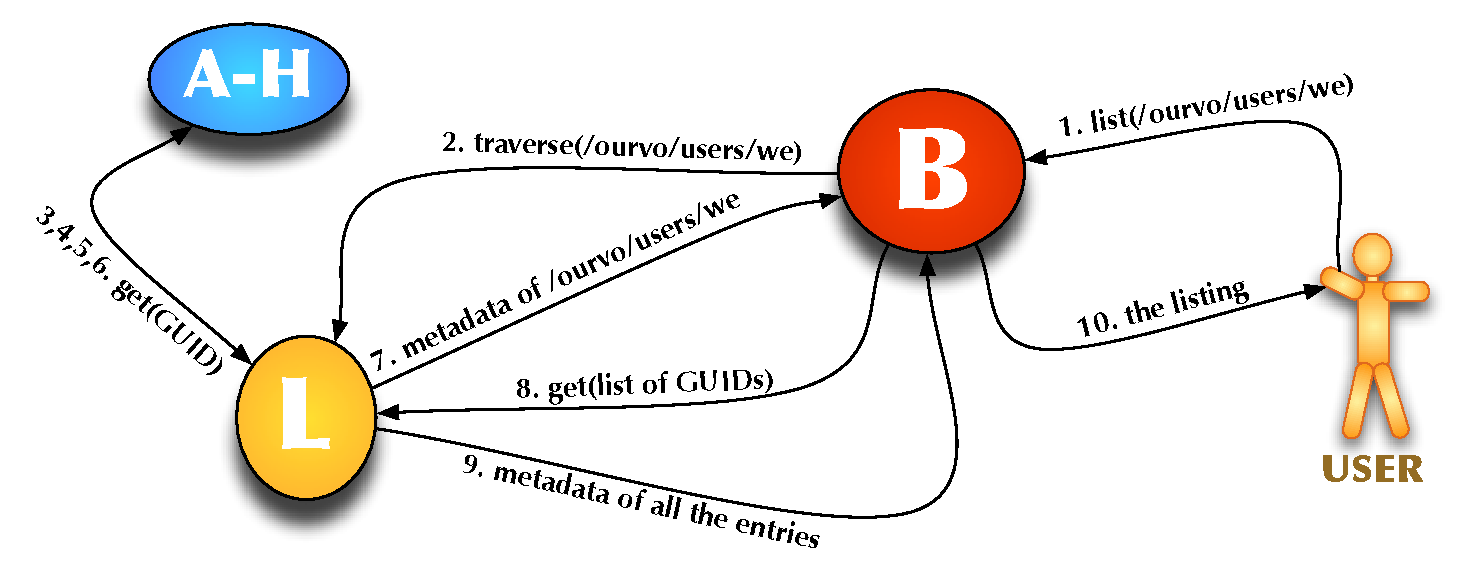
\includegraphics{arc-storage-listing.pdf}}}
\caption{\label{fig:listing}Listing the contents of a collection} }
\end{figure}

We want to list the contents of a collection, which has a Logical Name of \verb!/ourvo/users/we!. In order to do this, we have to contact a Bartender, and send a request to it containing the Logical Name we want to list, and the response from the Bartender will contain the list of entries. The steps are represented on Figure~\ref{fig:listing}.

\begin{enumerate}
    \item We need to know the URL of a Bartender. This could be preconfigured on the client side or in future releases it could be acquired from an information system. When we have the URL, we send a `list' request which contains the Logical Name \verb!/ourvo/users/we!.
    \item The Bartender tries to get the metadata of the given LN by sending a `traverseLN' request to a Librarian.
    \item The Librarian service starts the traversing by asking an A-Hash service about the first part of the LN, which is the \verb!/! root collection. The A-Hash service only knows about GUIDs and not about LNs, but the GUID of the root collection is well-known, so the A-Hash can return the metadata of it which contains the list of files and sub-collections in the root collection.
    \item Hopefully the \verb!ourvo! collection can be found in the root collection, which means that new the Librarian knows its GUID, and can ask for its metadata from the A-Hash.
    \item After the A-Hash returns the metadata of the \verb!/ourvo! collection, the Librarain finds the GUID of \verb!users! in it, then gets its metadata.
    \item The A-Hash returns the metadata of \verb!/ourvo/users! which contains the GUID of \verb!we!, so the Librarian can ask for its metadata.
    \item At last the A-Hash returns the metadata of \verb!/ourvo/users/we! to the Librarian, and the Librarian returns it to the Bartender. This metadata contains the list of entries within this collection, and it also contains the access policies for this collection.
    \item The Bartender first checks if based on our DN (or our VO membership) and the access policies of this collection do we have rights to get the contents of this collection or not. If we are approved, then because the `list' request should return additional metadata about each entry in the collection, the Bartender send a `get' message to a Librarian requesting metadata of all the entries in this collection.
    \item The Librarian gets the data from the A-Hash and returns it to the Bartender.
    \item Now the Bartender has all the needed information, so it could return the proper response to us, the user. Our client tool formats and prints the results nicely.
\end{enumerate}

% section listing_the_contents_of_a_collection (end)

\section{Downloading a file} % (fold)
\label{sec:downloading_a_file}
\begin{figure}[ht]
\centering{{\scalebox{0.7}{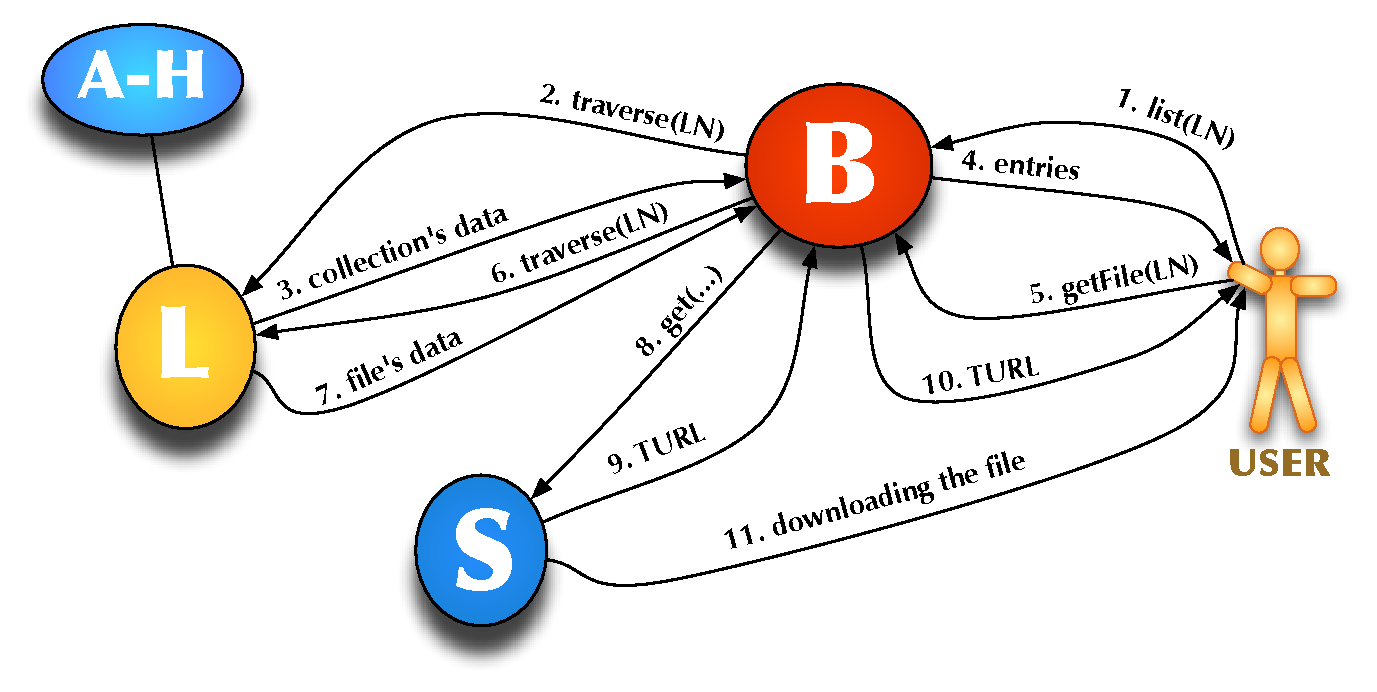
\includegraphics{arc-storage-downloading.pdf}}}
\caption{\label{fig:downloading}Downloading a file} }
\end{figure}

In this use case we want to download a file which has a Logical Name of \verb#/ourvo/users/we/thefilewewant# (see Figure~\ref{fig:downloading}).

\begin{enumerate}
    \item We connect a Bartender and send a `getFile' request with the LN of our file.
    \item The Bartender contacts a Librarian to traverse the Logical Name and to get the metadata of our file.
    \item The Librarian do the step by step traversing and gets all the data from the A-Hash and returns the metadata of our file to the Bartender. This metadata contains the location of the file's replicas and the access policies of this file.
    \item The Bartender checks based on the access policies and our identity if we are allowed to get the file, and if we are good to go, then it chooses a replica location. A location consists of the URL of a Shepherd service, and the ID of the replica within that Shepherd (which is called a `referenceID'). The Bartender sends a `get' request to the chosen Shepherd.
    \item The Shepherd prepares the file transfer by asking the storage element service to create a new one-time URL for this replica. This URL called the transfer URL, and it will only be valid for one download. The Shepherd returns the TURL to the Bartender.
    \item The Bartender returns the TURL to us.
    \item Now we use this TURL to get the file directly from the storage element service on the storage node.
\end{enumerate}

% section downloading_a_file (end)

\section{Creating a collection} % (fold)
\label{sec:creating_a_collection}
\begin{figure}[ht]
\centering{{\scalebox{0.7}{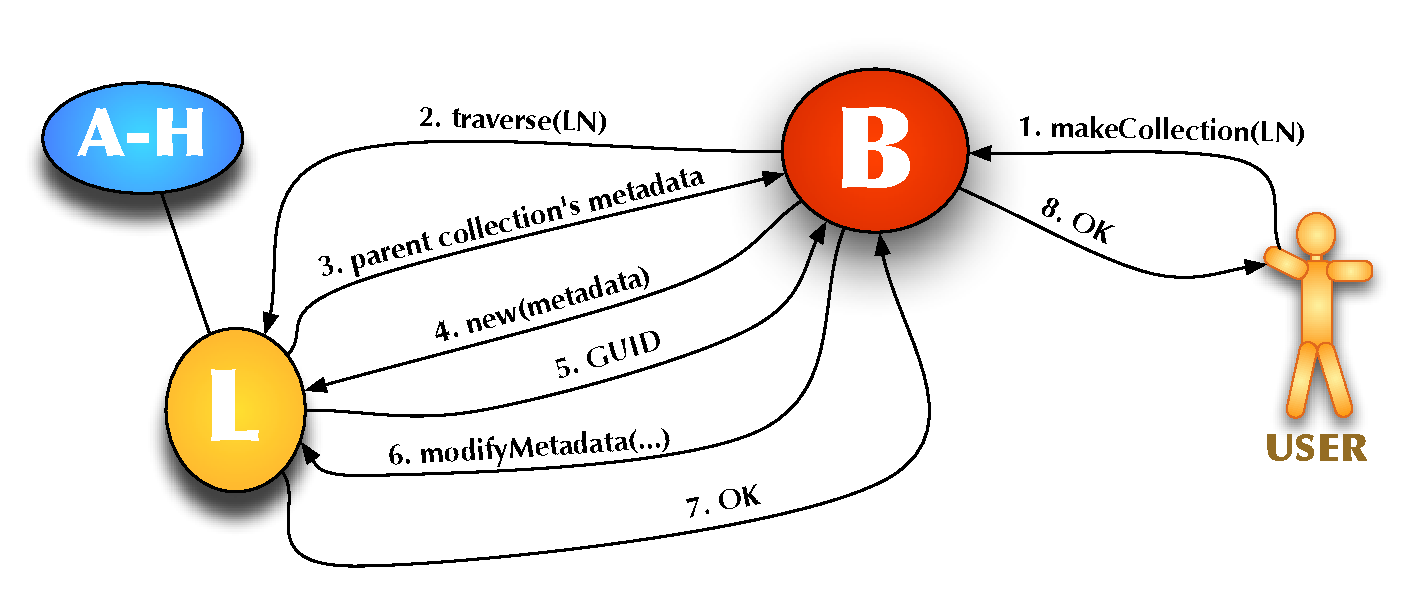
\includegraphics{arc-storage-makecollection.pdf}}}
\caption{\label{fig:makecollection}Creating a collection} }
\end{figure}

We want to create a new (empty) collection as sub-collection of \verb#/ourvo/common#, and we want to call it \verb!docs! (see Figure~\ref{fig:makecollection})

\begin{enumerate}
    \item We contact a Bartender and send a `makeCollection' request with the LN \verb!/ourvo/common/docs!.
    \item The Bartender asks a Librarian to traverse this LN.
    \item The Librarian try to traverse the Logical Name and it stops at the last possible point and returns the metadata of the last element. Because we want to put our collection to a new path but into an existing collection, we expect that only the \verb#/ourvo/common# part of the LN can be traversed. If the Librarian could traverse the whole LN that would mean that there is already an existing file or collection by that name. If the parent collection does exist then the Librarian can traverse it which means that the parent collection's metadata is returned to the Bartender. 
    \item The Bartender checks the access policies to decide if we have permissions to put something into this collection. Then it asks the Librarian to create a new collection.
    \item The Librarian creates the collection, and returns its GUID. At this point this new collection has no real Logical Name yet, it only has a GUID, but it is not yet put into its parent collection.
    \item The Bartender now asks the Librarian to add this new entry into the parent collection, which means that the new GUID and the name \verb!docs! are added as a pair.
    \item The Librarian returns with a status message.
    \item Finally the Bartender tells us if everything went OK or not.
\end{enumerate}


% section creating_a_collection (end)

\section{Uploading a file} % (fold)
\label{sec:uploading_a_file}

\begin{figure}[ht]
\centering{{\scalebox{0.7}{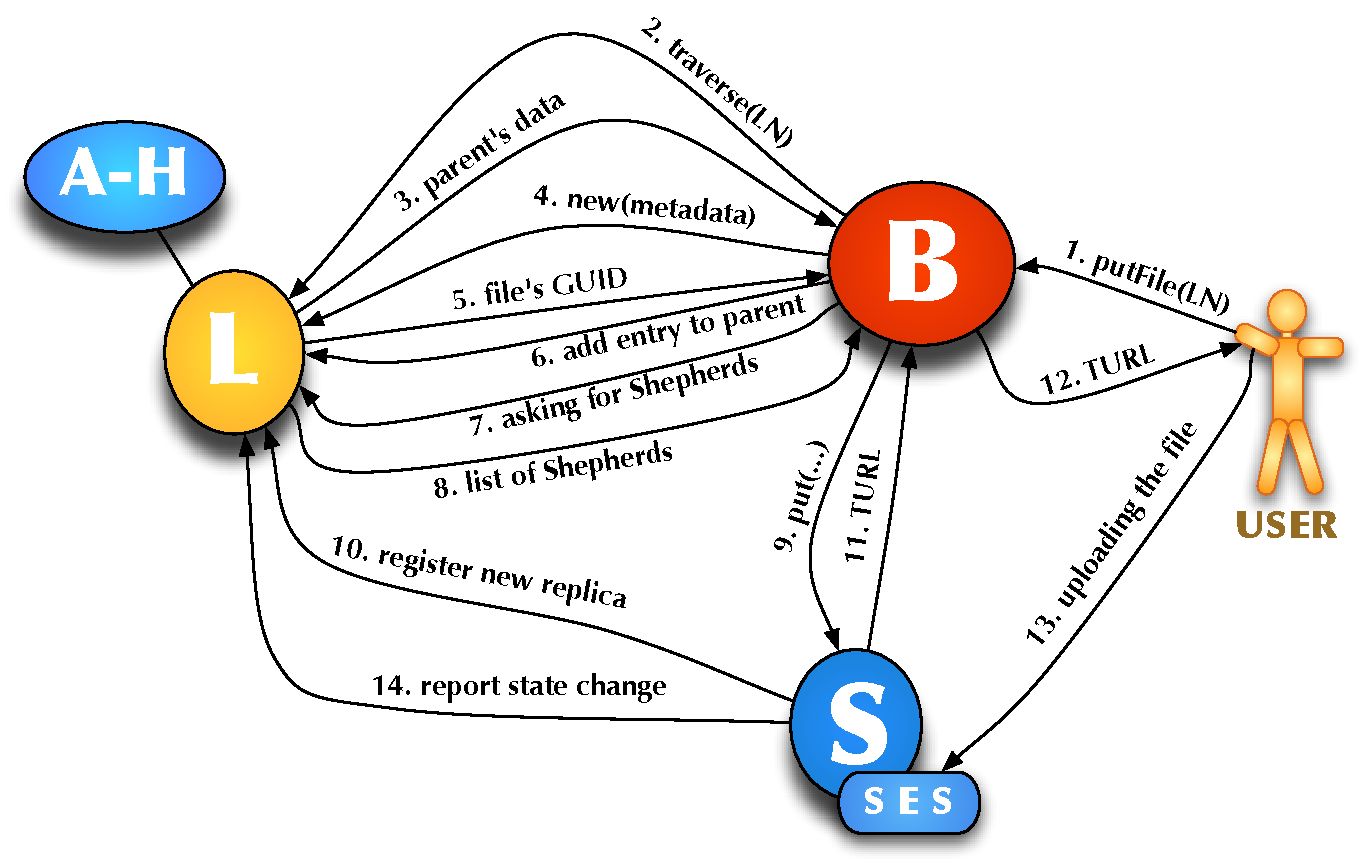
\includegraphics{arc-storage-uploading.pdf}}}
\caption{\label{fig:uploading}Uploading a file} }
\end{figure}

We have a file on our local disk we want to upload to a collection called \verb#/ourvo/common/docs#. (See Figure~\ref{fig:uploading}.)
\begin{enumerate}
    \item We contact a Bartender to put the file, we give the size and checksum and other metadata. And of course we give the Logical Name where we want to put the file, which in this case will be \verb#/ourvo/common/docs/proposal.pdf#
    \item The Bartender ask a Librarian to traverse this LN.
    \item The Librarian traverses the Logical Name, and we expect it to stop at the \verb#/ourvo/common/docs# part of the LN, because that means that the name is available and the parent collection exists. If everything is fine, the metadata of the parent collection is returned to the Bartender. 
    \item The Bartender checks the access policies to decide if we have permissions to put something into this collection. Then it asks the Librarian to create a new file entry. 
    \item The Librarian creates the entry and returns its GUID.
    \item Then the Bartender add the name \verb#proposal.pdf# and the new GUID to the collection \verb#/ourvo/common/docs# and from now on there will be a valid LN \verb#/ourvo/common/docs/proposal.pdf#. However this LN points to a file which has currently no replica at all. If someone tried to download the file called \verb#/ourvo/common/docs/proposal.pdf# now, would get an error message.
    \item The Bartender asks the Librarian about Shepherd services (which are sitting on storage nodes).
    \item The Librarian returns a list of Shepherd services
    \item The Bartender chooses a Shepherd service and sends it a `put' request to initiate the file upload. 
    \item The Shepherd communicates with the storage element service on the same node to create a new transfer URL (TURL). Then it creates a `referenceID' for this file and then reports to the Librarian that there is a new replica in \verb#creating# state. The Librarian gets the message from the Shepherd and adds the new replica to our new file. Now the file has one replica, which is not uploaded yet into the system. If someone tries to download this file now, still gets an error message.
    \item The Shepherd returns the the TURL to the Bartender.
    \item The Bartender returns the TURL to us.
    \item Then we can upload the file to this TURL.
    \item The Shepherd detects that the file is arrived. It checks the checksum of the file, and if it is OK, then it reports to the Librarian, that this replica is now \verb#alive#. The Librarian alters the state of this location, and now finally the file has one valid replica. 
\end{enumerate}
í
% section uploading_a_file (end)

\section{Removing a file} % (fold)
\label{sec:removing_a_file}

\begin{figure}[ht]
\centering{{\scalebox{0.7}{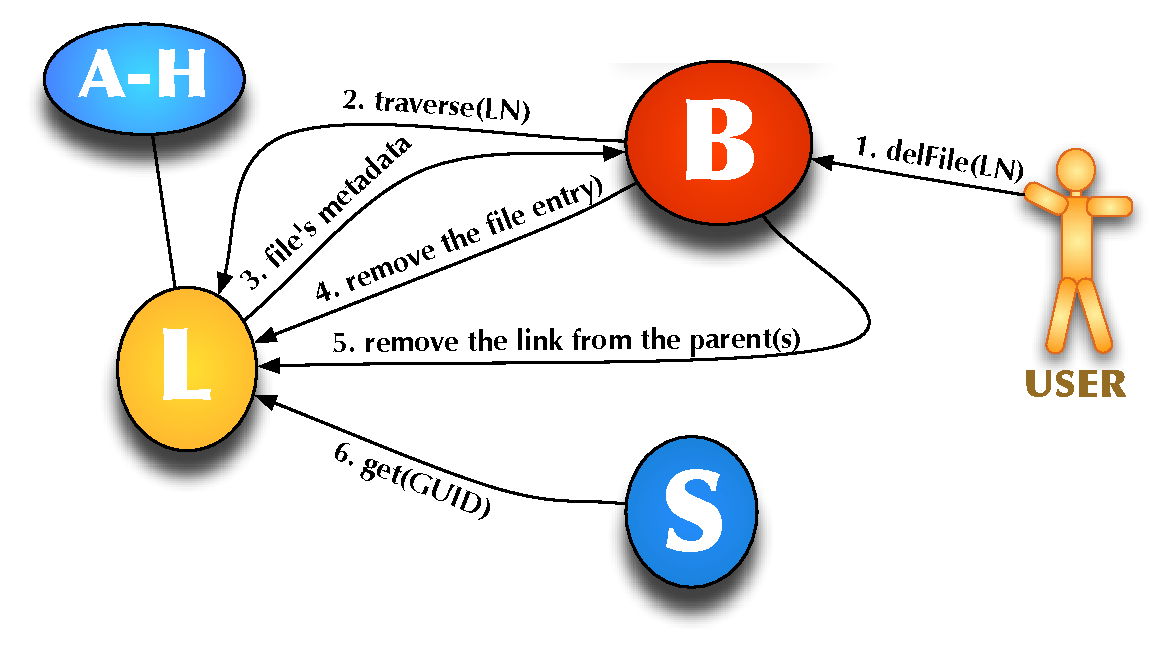
\includegraphics{arc-storage-removing.pdf}}}
\caption{\label{fig:removing}Removing a file} }
\end{figure}
\begin{enumerate}
    \item If we want to remove a file, we should connect to a Bartender with the LN of the file we want to remove.
    \item The Bartender asks the Librarian to traverse the LN.
    \item The Librarian returns the metadata of the file. The metadata contains information about all the hardlinks which points to this file if there are more than one.
    \item Now the Bartender asks the Librarian to remove the file.
    \item After that, the Bartender asks the Librarian to remove the links to this file from all the parent collections.
    \item Next time a Shepherd which has a replica of this file does its periodic check, it asks the Librarian about the file, and notices that the file does not exist anymore, so it removes the replica itself from the storage node.
\end{enumerate}


% section removing_a_file (end)

% chapter use_cases (end)

\chapter{Technical description} % (fold)
\label{cha:technical_description}

\section{Framework and language} % (fold)
\label{sec:framework_and_language}

The services are written in Python and running in the HED\footnote{The ARC container - \url{https://www.knowarc.eu/documents/Knowarc\_D1.2-2\_07.pdf}} hosting environment. The HED itself is written in C++, but there are language bindings which allow us to write services in other languages, e.g.~in Python or Java. The source code of the storage services are in the NorduGrid Subversion repository\footnote{\url{http://svn.nordugrid.org/trac/nordugrid/browser/arc1/trunk/src/services/storage}}.

Because the next-generation information system of ARC is currently under development, we cannot use it to discover services, that's why currently the URLs of almost all the services are hardcoded in the configuration files of the service. There is one exception: the Shepherd services are reporting their URLs to the Librarians, so a Bartender always could get a very current list of alive Shepherd services.

The HED also has a security framework which the Bartenders use the make access policy decision . The details of this is described in section X.

% section framework_and_language (end)

\section{Data model} % (fold)
\label{sec:data_model}

The ARC storage system stores different kinds of metadata about files, collections, mount point, Shepherd services, etc. Each of these has a unique ID which we call `GUID'.

The A-Hash services provide a functionality to store `objects', where each object has a unique ID, and contains key-value pairs organized in sections. The properties, the values and the section names too are simple character strings. The A-Hash services provide a simple interface to interact with these objects, e.g.~to do conditinal and atomic changes.

The Librarian services use the A-Hash services to store the metadata of all kinds, using the GUIDs as unique IDs. For this, we have to represent the metadata as key-value pairs organized in section. The files, the collections and the mount points have some common attributes: the GUID, the type and the owner which are in the \emph{entry} section; the creation and modification timestamps in the \emph{timestamps} section, a list of access control rules in the \emph{policy} section; the list of parent collections where this entry has a `hardlink'; and each entry could have arbitrary key-value pairs in the \emph{metadata} section.

\begin{description}
    \item [entry] section 
    \begin{itemize}
        \item \emph{type}: the type of the entry: `collection', `file' or `mountpoint'
        \item \emph{GUID}: the unique ID of the entry
        \item \emph{owner}: the DN of the user how ownes this entry
    \end{itemize}
    \item [timestamps] section 
    \begin{itemize}
        \item \emph{created}: timestamp of creation 
        \item \emph{modified}: timestamp of last modification (the support for this is not implemented yet)
    \end{itemize}
    \item [policy] section 
    \begin{itemize}
        \item \emph{(identity, action list) pairs}: a list of allowed and not allowed actions for different identites (users, VOs, etc.). 
    \end{itemize}
    \item [parents] section
    \begin{itemize}
        \item list of GUIDs of collection where this entry is located, and the name of this entry within the given collections
    \end{itemize}
    \item [metadata] section 
    \begin{itemize}
        \item any other arbitrary key-value pairs
    \end{itemize}
\end{description}

\subsection{Files} % (fold)
\label{sub:files}

A file in the ARC storage has a logical entry in the namespace, and a couple of physical replicas on the storage nodes. We store the locations of the replicas in the \emph{location} section. A location contains the URL of the Shepherd service, the local ID of the file within the storage node and the state of the replica. This state could be `\textbf{alive}' (if the replica passed the checksum test, and the Shepherd reports that the storage node is healthy), `\textbf{invalid}' (if the replica has wrong checksum, or the Shepherd claims it has no such file), `\textbf{offline}' (if the Shepherd is not reachable, but may have a valid replica), `\textbf{creating}' (if the replica is in the state of uploading), `\textbf{thirdwheel}' (if the replica is marked for deletion because of too many replicas). We also store (in the \emph{states} section) the size of the file, the number of needed replicas, and a checksum of the file, which is created by some kind of checksuming algorithm (currently only md5 is supported).

\begin{description}
    \item [locations] section 
    \begin{itemize}
        \item \emph{(location, state) pairs}, where a location is a (\emph{URL}, \emph{referenceID}) pair serialized as a string, where \emph{URL} is the address of the Shepherd service storing this replica, \emph{referenceID} is the ID of the file within that Shepherd service.
    \end{itemize}
    \item [states] section 
    \begin{itemize}
        \item \emph{size}: the file size in bytes
        \item \emph{checksum}: checksum of the file
        \item \emph{checksumType}: the name of the checksum method
        \item \emph{neededReplicas}: how many valid replicas should this file have 
    \end{itemize}
\end{description}


% subsection files (end)


% The Librarian uses the A-Hash to store all the data about files and collections. The A-Hash is capable of storing key-value pairs organized in sections, which actually means that it stores (\emph{section}, \emph{key}, \emph{value}) tuples where each member is simply a string, e.g.~(`entry', `type', `collection') or (`ACL', `johnsmith', `owner') or (`timestamps', `created', `1196265901') or (`locations', `64CDF45F-DDFA-4C1D-8D08-BCF7810CB2AB:9A293F27DC86', `sentenced'). There could be only one \emph{value} for a (\emph{section}, \emph{key}) pair.


\subsection{Collections} % (fold)
\label{sub:collections}

A \emph{collection} is a list of files and other collections, which are in parent-children relationships forming a tree-hierarchy. Each entry has a unique name within a collection and a GUID which points to corresponding file or collection, so a collection is basically a list of name-GUID pairs, which list is stored in the \emph{entries} section. The collections could be in a closed state, which means that its contents should not be changed. If you close a collection then it cannot be opened again. However it cannot be garanteed that the contents of a closed collection remains the same (e.g. if we include in our collection a file which we don't own, then the owner of the file could remove it nevertheless), but if a closed collection is changed, its state will be broken, and this state could never be changed again, which means you will always know if a closed collection is not intact anymore. This state is stored in the \emph{states} section, and its values could be `\textbf{no}' (if the collection is not closed), `\textbf{yes}' (if the collection is closed) and `\textbf{broken}' (if the collection was closed, but something happened, and its contents have been changed).

\begin{description}
    \item [entries] section 
    \begin{itemize}
        \item \emph{(name, GUID) pairs}: a collection is basically a list of name-GUID pairs. 
    \end{itemize}
    \item [states] section 
    \begin{itemize}
        \item \emph{closed}: this indicates if the collection is closed or broken. 
    \end{itemize}
\end{description}

% subsection collections (end)

\subsection{Mount Points} % (fold)
\label{sub:mount_points}

The mount point entry is a reference to an external third-party storage. Its metadata is basically just the URL of the external storage.

\begin{description}
    \item [mountpoint] section 
    \begin{itemize}
        \item \emph{externalURL}: the URL of the external storage.
    \end{itemize}
\end{description}


% subsection mount_points (end)

\subsection{Shepherds} % (fold)
\label{sub:shepherds}

The Librarian stores information about the registered Shepherd services. Each Shepherd reports its URL and the list of its files to a Librarian, and for each Shepherd a GUID is created. There is a special entry (with GUID `1' by default) which stores a list of the registered Shepherd services, storing their GUID and the timestamp of the last heartbeat message from them.

\begin{description}
	\item [nextHeartBeat] section
	\begin{itemize}
		\item (URL, timestamp) pairs contains when was the last heartbeat of this service
	\end{itemize}
	\item [serviceGUID] section
    \begin{itemize}
        \item (URL, GUID) pairs connects the URL of the Shepherd to the GUID where the information is stored about the Shepherd's stored files
    \end{itemize}
\end{description}

And for each Shepherd there is a separate entry with the list of all files stored on the given storage nodes:

\begin{description}
	\item [entry] section
    \begin{itemize}
        \item \emph{type}: `shepherd'
    \end{itemize}
	\item [files] section
	\begin{itemize}
	    \item \emph{(referenceID, GUID) pairs} for each replica stored on the Shepherd
	\end{itemize}
\end{description}

% subsection shepherds (end)


% section data_model (end)

\section{Security implementation} % (fold)
\label{sec:security_implementation}

The ARC HED hosting environment has a security framework, and it has its own policy language for describing access policies and requests. While the storage system use its own format to store the access policies, but one the time comes to make decision, it converts the stored policies and the incoming requests to this ARC native policy format, and uses the security framework to decide.

%%%%%%%%%%%%%%%%

% section security_implementation (end)

\newpage

\section{A-Hash} % (fold)
\label{sec:a_hash}

\subsection{Functionality} % (fold)

The A-Hash will be a distributed service capable of storing tuples of strings in a scalable manner. Currently it only has a centralized implementation. It stores \emph{objects}, where each object has an arbitrary string \emph{ID}, and contains any number of \emph{key}-\emph{value} pairs grouped in \emph{section}s, where \emph{key}, \emph{value} and \emph{section} are arbitrary strings. There could only be a single \emph{value} for a \emph{key} in a \emph{section}.

If you have an ID, you can get all key-value pairs of the corresponding object with the \emph{get} method, or you could specify only which sections or properties do you need. You can add or remove key-value pairs of an object or delete all occurrences of a key or create a new object with the \emph{change} method, and you can specify conditions, which means the change is only applied if the given conditions are met.

% subsection functionality (end)

\subsection{Prototype status and plans} % (fold)

The A-Hash service currently implemented as a single central service, which stores the data on disk in separate files per \emph{object}. Fall of 2008 it will be reimplemented using a distributed hash table (DHT) algorithm, one possible candidate is the Chord\footnote{The Chord project - \url{http://pdos.csail.mit.edu/chord/}} algorithm with a consistency solution called Etna\footnote{Etna: a Fault-tolerant Algorithm for Atomic Mutable DHT Data - \url{http://pdos.csail.mit.edu/\~athicha/papers/etna.ps}} on top of it. This reimplementation hopefully won’t change the interface of the service.

% subsection prototype_status_and_plans (end)

\subsection{Data model} % (fold)

\begin{itemize}
    \item \emph{ID} is an arbitrary string
    \item \emph{object} contains key-value pairs in sections, technically it is a list of key-\emph{value} pairs where the key is a (\emph{section}, \emph{key}) tuple
\end{itemize}

% subsection data_model (end)

\subsection{Interface} % (fold)

\begin{description}
    \item [get(ids, neededMetadata)] returns \emph{getResponse} which is a list of (\emph{ID}, \emph{object}) pairs.

    The \emph{ids} is a list of string \emph{ID}s, \emph{neededMetadata} is a list of (\emph{section}, \emph{key}) pairs. For each \emph{ID} it returns all the \emph{value}s for each \emph{key} in each \emph{section} (filtered by \emph{neededMetadata}), so \emph{object} is a list of (\emph{section}, \emph{key}, \emph{value}) tuples.

    \item [change(changeRequest)] returns \emph{changeResponse} which is a list of (\emph{changeID}, \emph{success}, \emph{failedConditionID}) tuples.

    \emph{changeRequest} is a tuple of (\emph{changeID}, \emph{ID}, \emph{changeType}, \emph{section}, \emph{key}, \emph{value}, \emph{conditions}), where \emph{changeID} is an arbitrary ID to identify in the response which change was successful; \emph{ID} points to the object we want to change; \emph{changeType} can be `\textbf{set}' (set the key within the section to value), `\textbf{unset}' (remove the key from the section regardless of the value), `\textbf{delete}' (removes the whole object), conditions is a list of (\emph{conditionID}, \emph{type}, \emph{section}, \emph{key}, \emph{value}) tuples, where \emph{type} could be `\textbf{is}' (the key in the section is set to the value), `\textbf{isnot}' (the key in the section is not set to the value), `\textbf{isset}' (the key of the section is set to any value), `\textbf{unset}' (the key of the section is not set at all).
    If all conditions are met, tries to apply changes to the objects, creates a new object if a previously non-existent ID is given. If one of the conditions is not met, returns the ID of the failed condition.
\end{description}
    
% subsection interface (end)

% section a_hash (end)
\newpage

\section{Librarians} % (fold)
\label{sec:librarian}

\subsection{Functionality} % (fold)
% 
The Librarian manages a tree-hierarchy of files, grouping them into collections. There is a root collection with a well-known GUID which can be used as starting point when resolving Logical Names. If you create a new collection with the method \emph{new}, the Librarian generates a new GUID, but does not insert it into the tree-hierarchy which can be done by adding this GUID as a new entry to one of the existing collection using the \emph{modifyMetadata} method of the existing collection which makes it the parent of the new collection. A collection can be closed via metadata modification which cannot be undone and prevents files to be added or removed from this collection. A new file  also can be created with the \emph{new} method which returns the newly generated GUID of the new file entry which should be added to a parent collection to insert it into the global namespace. A file has a list of locations where its replicas are stored, this list too can be manipulated with \emph{modifyMetadata}. The access policies of the files and collections are also stored as metadata. The \emph{remove} method deletes an entry from the Librarian. The \emph{traverseLN} method try to traverse Logical Names by walking the hierarchy of the namespace and to return the GUID of the entry pointed by the LN. After you have a GUID of file, collection or mount point, you can get all the information using the \emph{get} method. 

% subsection functionality (end)

\subsection{Prototype status and plans} % (fold)

The Librarian service currently implements all the methods below, but doesn't do very much error checking. This should be changed, the Librarian should check the validity of metadata, and forbid some cases, e.g.~reopen a closed collection.

% subsection prototype_status_and_plans (end)

\subsection{Data model} % (fold)
\label{sub:data_model}

% subsection data_model (end)

\subsection{Interface} % (fold)

 \begin{description}
    \item[new(newRequestList)] returns a list of (\emph{requestID}, \emph{GUID}, \emph{success})
    
    \emph{newRequestList} is a list of (\emph{requestID}, \emph{metadata}) where \emph{requestID} is an arbitrary ID used to identify this request in the list of responses; \emph{metadata} is a list of (\emph{section}, \emph{key}, \emph{value}) tuples.
    This method generates a \emph{GUID} for each request, and inserts the new entry (with the given metadata) into the A-Hash, then returns the GUIDs of the newly created entries. The (`entry', `type') key of the metadata contains whether it is a file or a collection.
    
    \item[modifyMetadata(modifyMetadataRequestList)] returns a list of (\emph{changeID}, \emph{success})

    \emph{modifyMetadataRequestList} is a list of (\emph{changeID}, \emph{GUID}, \emph{changeType}, \emph{section}, \emph{key}, \emph{value}) where \emph{changeType} can be `\textbf{set}' (set the key in the section to value), `\textbf{unset}' (remove the key-value pair from the section), `\textbf{add}' (set the key in the section to value only if it is not exists already).
    
    \item [get(GUIDs, neededMetadata)] returns \emph{getResponse}
    
    \emph{GUIDs} is a list of GUIDs, \emph{neededMetadata} is a list of (\emph{section}, \emph{key}) pairs indicating only which properties we need, \emph{getResponse} is a list of (\emph{GUID}, \emph{metadata}) where metadata is a list of (\emph{section}, \emph{key}, \emph{value}) tuples. This method returns the metadata of all the \emph{GUID}s filtered with \emph{neededMetadata}.
    
    \item [remove(removeRequestList)] returns a list of (\emph{requestID}, \emph{success}) pairs
    
    \emph{removeRequestList} is a list of (\emph{requestID}, \emph{GUID}) pairs. \emph{success} could be `\textbf{removed}' or `\textbf{failed}: reason'.
    
    \item [traverseLN(traverseRequestList)] returns \emph{traverseResponseList}
    
    \emph{traverseRequestList} is a list of (\emph{requestID}, \emph{LN}) with the Logical Names to be traversed
    
    \emph{traverseResponseList} is a list of (\emph{requestID}, \emph{metadata}, \emph{GUID}, \emph{traversedLN}, \emph{restLN}, \emph{wasComplete}, \emph{traversedList}) where:
    \begin{description}
        \item[metadata] is all the metadata of the of traversedLN in the form of (\emph{section}, \emph{key}, \emph{value}) tuples
        \item[GUID] is the \emph{GUID} of the \emph{traversedLN}
        \item[traversedLN] is the part of the \emph{LN} which was traversed, if \emph{wasComplete} is true, this should be the full \emph{LN}
        \item[restLN] is the postfix of the \emph{LN} which was not traversed for some reason, if \emph{wasComplete} is true, this should be an empty string
        \item[wasComplete] indicates whether the full \emph{LN} was traversed
        \item[traversedList] is a list of (\emph{LNpart}, \emph{GUID}) pairs, where \emph{LNpart} is a part of the \emph{LN}, \emph{GUID} is the GUID of the Librarian-entry referenced by that part of the \emph{LN}, the first element of this list is the shortest prefix of the \emph{LN}, the last element is the \emph{LN} without its last part
    \end{description}
    
    \item [report(serviceID, filelist)] returns in \emph{nextReportTime} a number of seconds, which is the timeframe within the Librarian expects the next heartbeat from the Shepherd
    
    \emph{filelist} is a list of (\emph{GUID}, \emph{referenceID}, \emph{state}) tuples containing the state of changed or new files, where \emph{state} could be `\textbf{invalid}' (if the periodic self-check of the Shepherd found a non-matching checksum or missing file), `\textbf{creating}' (if this is a new file not uploaded yet) or `\textbf{alive}' (if the file is uploaded and the checksum is OK).
    
\end{description}


% subsection interface (end)

% section librarian (end)
\newpage

\section{Shepherds} % (fold)
\label{sec:shepherds}

\subsection{Functionality} % (fold)

A Shepherd service is capable of managing a storage node. It keeps track all the files it stores with their GUIDs and checksums. It periodically checks each file to detect corruption, and send reports to a Librarian indicating that the storage node is up and running, and whether some file's state has been changed. If a file goes missing or has a bad checksum then the Librarian is notified about the error (here the Shepherd refers to the file with its GUID, that's why it needs to store the GUIDs of its files). It periodically asks the Librarian how many replicas its files have, and if a file has fewer replicas than needed, the Shepherd offers its copy for replication by calling the Bartender.

A Shepherd service is always connected to a file transfer service (e.g.~`HTTP(S)', `FTP(S)', `ByteIO', `GridFTP', etc.). For each supported file transfer service we need a backend module which makes the Shepherd capable of communicating with the file transfer service to initiate file transfers, to detect whether a transfer was successful or not, to generate local IDs and checksums, etc.

A file in a storage node could be identified with a \emph{referenceID} which is unique within that node. If we know the \emph{location} of a file, which is the ID of the Shepherd service (\emph{serviceID}) and the \emph{referenceID}, we could get the endpoint reference (URL) of the Shepherd from the information system, then we could call its \emph{get} method with the \emph{referenceID} and a list of transfer protocols we can use (e.g.~`HTTP', `FTP'), the Shepherd chooses a protocol from this list which it can provide, and create a transfer URL (\emph{TURL}) and returns it along with the \emph{checksum} of the file. We could download the file from this \emph{TURL}, and verify it with the \emph{checksum}. An end user of the storage system does not need to call this \emph{get} method, because the Bartender service will do it, the user just asks the Bartender and gets the TURL.

Storing a file starts with initiating the transfer with the \emph{put} method of the Shepherd, we should give the \emph{size} and \emph{checksum} of the file and its \emph{GUID} as well. We also specify a list of transfer protocols we are able to use, and the Shepherd chooses a \emph{protocol}, creates a \emph{TURL} for uploading and generates a \emph{referenceID}, then we can upload the file to the TURL. Again, the end user just asks the Bartender, and gets the TURL, the user does not need to call the \emph{put} method of the Shepherd directly.

These \emph{TURL}s are one-time URLs which means that after the client uploads or downloads the file these \emph{TURL}s cannot be used again to do the same. If we want to download the same file twice, we have to initiate the transfer twice, and will get two different \emph{TURL}s.

With the \emph{stat} method we can get some information about a replica, e.g.~checksum, GUID, state (`creating', `alive' or `invalid'), etc. The \emph{delete} method removes the file.

In normal operation the \emph{put} and \emph{get} calls is made by a Bartender but the actual uploading and downloading is done by the user's client. In the case of replication a Shepherd with a valid replica initiates the replication, this Shepherd asks the Bartender to choose a new Shepherd, the Bartender initiates putting the new replica on a chosen Shepherd and receives the TURL, then the Bartender returns the TURL to the initiator Shepherd, which uploads its replica to the given TURL.

% subsection functionality (end)

\subsection{Prototype status and plans} % (fold)

The current implementation of the Shepherd service has a working \emph{get}, \emph{put}, \emph{stat}, \emph{delete} methods, and a method called \emph{toggleReport} which can be used the simulate storage node failure with the Shepherd not reporting to a Librarian. 
There is a separate service which provide a subset of the ByteIO interface, and there is an other separate service which is a basic HTTP server, these are both could be used as file transfer services, both have its backend module for the Shepherd. Currently both file transfer services have the problem of using too much memory while transferring files.
Further plans include better file transfer services and backend modules for third-party file transfer services.

% subsection prototype_status_and_plans (end)

\subsection{Data model} % (fold)

A file of a Shepherd service is referenced by its \emph{referenceID}. Each file has a \emph{state} which could be `\textbf{creating}' when the transfer is initiated but the file is not uploaded yet, `\textbf{alive}' if the file is uploaded and has a proper checksum, or `\textbf{invalid}' if it does not exists anymore or has a bad checksum. Each file has a \emph{localID} which is used in the backend modules.

% subsection data_model (end)



\subsection{Interface} % (fold)

\begin{description}
    \item[get(getRequestList)] returns list of (\emph{requestID}, \emph{getResponseData})
    
    \emph{getRequestList} is a list of (\emph{requestID}, \emph{getRequestData}) where \emph{requestID} is an arbitrary ID used in the reply
    
    \emph{getRequestData} is a list of (\emph{key}, \emph{value}) pairs, where mandatory properties are: `\textbf{referenceID}' which refers to the file to get and `\textbf{protocol}' indicates a protocol the client can use (there could be multiple protocols in getRequestData).
    
    \emph{getResponseData} is a list of (\emph{key}, \emph{value}) pairs, such as: `\textbf{TURL}' is a transfer URL which can be used by the client to download the file; `\textbf{protocol}' is the protocol of the TURL; `\textbf{checksum}' is the checksum of the replica; `\textbf{checksumType}' is the name of the checksum method and `\textbf{error}' could contain an error message if there is one.
     
    \item[put(putRequestList)] returns a list of (\emph{requestID}, \emph{putResponseData})
    
    \emph{putRequestList} is a list of (\emph{requestID}, \emph{putRequestData}) where \emph{requestID} is an ID used for the response
    
    \emph{putRequestData} is a list of (\emph{key}, \emph{value}) pairs such as `\textbf{GUID}', `\textbf{checksum}', `\textbf{checksumType}', `\textbf{size}' (the size of the file in bytes), `\textbf{protocol}' (a protocol the client can use, can be multiple) and `\textbf{acl}' (for additional access policy).
    
    \emph{putResponseData} is a list of (\emph{key}, \emph{value}) pairs such as: `\textbf{TURL}' is the transfer URL where the client can upload the file, `\textbf{protocol}' is the chosen protocol of the TURL and `\textbf{referenceID}' is the generated ID for this new replica, `\textbf{error}' could contain an error message.
    
    \item[delete(deleteRequestList)] returns a list of (\emph{requestID}, \emph{status})
    
    \emph{deleteRequestList} is a list of (\emph{requestID}, \emph{referenceID}) pairs selecting the files to remove. The status could be `\textbf{deleted}' or `\textbf{nosuchfile}'
    .
    \item[stat(statRequestList)] returns a list of (\emph{requestID}, \emph{referenceID}, \emph{state}, \emph{checksumType}, \emph{checksum}, \emph{acl}, \emph{size}, \emph{GUID}, \emph{localID})
    
    \emph{statRequestList} is a list of (\emph{requestID}, \emph{referenceID}) where \emph{referenceID} points to the file whose data we want to get. The method returns all the data the Shepherd know about the replica.
     
\end{description}

% subsection interface (end)

\subsection{Backend modules} % (fold)
\label{sub:backend_modules}

The Shepherd could communicate with the file transfer services via backend modules. Currently there are two kinds of backend modules, one for the \emph{byteio} service (which is a simple implementation of a subset of the ByteIO interface) and one for the \emph{Hopi} service (which is a simple HED-based HTTP server).

In both cases the Shepherd and the transfer services should have access to the same local filesystem where the Shepherd creates two separate directories: one for storing all the files (e.g.~\verb!./store!) and one for the file transfers (e.g.~\verb!./transfer!). The store directory always contains all the files the Shepherd manages, the transfer directory is empty at the beginning.

Let's see the scenario for the Hopi service which should be in a special `slave' mode for this kind of operation: if a client asks for a file called \verb!file1!, and this file is in the store directory (\verb!./store/file!), then the Shepherd service creates a hardlink into the transfer directory (e.g.~\verb!./transfer/abc!) and sets this file read-only. If the Hopi service is configured that way that it handles the HTTP path \verb!/prb! and it is serving files from the directory \verb!./transfer! then after the hardlink is created, we have this URL for this file: \verb!http://localhost:60000/prb/abc!. Now we can give this URL to the client. Then the client \verb!GET!s this URL and gets the file. The Hopi service removes (unlinks) this file immediately after the \verb!GET! request arrived, which makes this \verb!http://localhost:60000/prb/abc! URL invalid (so this is a one-time URL), but because of the hardlink the file is still there in the store directory, it is just removed from the transfer directory. Now if some other user wants this file, the Shepherd creates an other hardlink, e.g.~\verb!./transfer/qwe! and now we have an URL \verb!http://localhost:60000/prb/qwe!.

If a client wants to upload a new file, then the Shepherd creates an empty file in the store directory, e.g.~\verb!./store/file2! and creates a hardlink into the transfer directory, e.g.~\verb!./transfer/oiu! and makes it writable, and now we have a URL \verb!http://localhost:60000/prb/oiu!, and the client is able to do a \verb!PUT! to this URL. When the client \verb!PUT!s the file there, the Hopi service immediately removes the uploaded file from the transfer directory, but because it has a hardlink in the store directory, the file is stored there as \verb!./store/file2!. The backend module for the Hopi service periodically checks whether a new file has two or just one hard links. If it has only one that means that a file is uploaded, so it could notify the Shepherd that the file is arrived. In order to do that, all the backend modules get a callback method `file\_arrived' from the Shepherd.

In case of the byteio service, there is some small differences. The byteio service does not removes the files from the transfer directory, but it calls the backend module via SOAP to notify it that something is happened. The byteio backend has one SOAP method called `\textbf{notify}':
\begin{description}
    \item[notify(subject, state)] returns `\textbf{OK}' in \emph{notifyResponse}.
\end{description}
When this method is called, the byteio backend module notifies the Shepherd that the file is arrived.

All the backend modules should have this common interface which the Shepherd can use to communicate with the file transfer service:
\begin{description}
    \item[prepareToGet(referenceID, localID, protocol)] returns the \emph{TURL}.
    
    Initiate transfer with \emph{protocol} for the file which has these IDs: \emph{localID} and \emph{referenceID}. The reason for including here the referenceID as well is that this information could be used by the backend module later, e.g.~when the transfer finished and the state of the file needs to be changed.
    
    \item[prepareToPut(referenceID, localID, protocol)] returns the \emph{TURL}.
    
    Initiate transfer with \emph{protocol} for the file which has these IDs: \emph{localID} and \emph{referenceID}.
    
    \item[copyTo(localID, turl, protocol)] returns \emph{success}.
    
    Upload the file referenced by \emph{localID} to the given \emph{TURL} with the given \emph{protocol}.
    
    \item[copyFrom(localID, turl, protocol)] returns \emph{success}.
    
    Download the file from the given \emph{TURL} with the given \emph{protocol}, and store it as \emph{localID}.
    
    \item[list()] returns a list of \emph{localID}s currently in the store directory.
    \item[getAvailableSpace()] returns the available disk space in bytes.
    \item[generateLocalID()] returns a new unique \emph{localID}.
    \item[matchProtocols(protocols)] only leave that protocols in the list \emph{protocols} which are supported by this file transfer service.
    \item[checksum(localID, checksumType)] returns the checksum of the file referenced by \emph{localID}, which checksum is generated by the method \emph{checksumType}.
     
\end{description}

% subsection backend_modules (end)

% section shepherds (end)
\newpage

\section{Bartenders} % (fold)
\label{sec:bartenders}

\subsection{Functionality} % (fold)

The Bartender provides an easy to use interface of the ARC storage system to the users. You can put, get and delete files using their logical names (\emph{LN}s) with the \emph{putFile}, \emph{getFile} and \emph{delFile} methods, create, remove and list collections with \emph{makeCollection}, \emph{unmakeCollection} and \emph{list}. The metadata of a file or collection (e.g.~whether the collection is closed, number of needed replicas, access policies) can be changed with \emph{modify}. A \emph{stat} call gives all the information about a file or collection, and you can move (or hardlink) collections and files within the namespace with \emph{move}. You can upload an entirely new replica to a file (e.g.~if the file lost all its replicas, or when a Shepherd service offers its replica for replications) with \emph{addReplica}.

% subsection functionality (end)

\subsection{Prototype status and plans} % (fold)

The methods mentioned in the above section are all implemented, but need more error-checking and metadata-checking. There are plans of adding new methods, e.g.~a \emph{copy} method or a \emph{glob} method for file pattern matching. The current version does not support closed (unmodifiable) collections yet.

% subsection protoype_status_and_plans (end)

\subsection{Data model} % (fold)

The Bartender interface uses mostly Logical Names (\emph{LN}s), which have the syntax of: \verb!<GUID>/<path>! where both sides can be omitted (and in the case of a sole GUID we don't need the slash either), e.g.~\verb!afg342/foo! is an entry called \verb!foo! in the collection with GUID \verb!afg342!; the LN \verb!f36a7481! refers to the a file or collection with GUID \verb!f36a7481!; \verb!/vo/dir/stg! points to the entry which is reachable from the root collection using the given path; and \verb!/! simply refers to the root collection.
The term `\emph{metadata}' here refers to a list of key-value pairs organized in sections, see the data model description in Section~\ref{sub:data_model}.

% subsection data_model (end)

\subsection{Interface} % (fold)

\begin{description}
    \item[putFile(putFileRequestList)] returns a list of (\emph{requestID}, \emph{success}, \emph{TURL}, \emph{protocol})
    
    \emph{putFileRequestList} is a list of (\emph{requestID}, \emph{LN}, \emph{metadata}, \emph{protocols}), where \emph{requestID} is an arbitrary ID which will be used in the response; \emph{LN} is the chosen Logical Name of the new file, \emph{protocols} is a list of protocols we can use for uploading, \emph{metadata} is a list of (\emph{section}, \emph{key}, \emph{value}) tuples where properties could be in the `\textbf{states}' section: `\textbf{size}', `\textbf{checksum}', `\textbf{checksumType}', and  `\textbf{neededReplicas}', policy documents in the `\textbf{policies}' section and any other key-value pairs in the `\textbf{metadata}' section. The returned \emph{TURL} is a URL with a chosen \emph{protocol} to upload the file itself, the \emph{success} string could be `\textbf{done}', `\textbf{missing metadata}', `\textbf{parent does not exists}', `\textbf{internal error:} reason', etc.

    \item[getFile(getFileRequestList)] returns a list of (\emph{requestID}, \emph{success}, \emph{TURL}, \emph{protocol})

    \emph{getFileRequestList} is a list of (\emph{requestID}, \emph{LN}, \emph{protocols}) where \emph{requestID} is used in the response, \emph{LN} is the Logical Name referring to the file we want to get, \emph{protocols} is a list of transfer protocols the client supports.
    In the response \emph{TURL} is the transfer URL using \emph{protocol}, with which we can download the file, \emph{success} could be `\textbf{done}', `\textbf{not found}', `\textbf{is not a file}', `\textbf{file has no valid replica}', `\textbf{error while getting TURL:} reason', etc.

    \item[delFile(delFileRequestList)] returns a list of (\emph{requestID}, \emph{status})
    
    \emph{delFileRequestList} is a list of (\emph{requestID}, \emph{LN}) with the Logical Name of the file we want to delete. The status in response could be `\textbf{deleted}' or `\textbf{nosuchLN}'.
    
    \item[stat(statRequestList)] returns a list of (\emph{requestID}, \emph{metadata})
    
    \emph{statRequestList} is a list of (\emph{requestID}, \emph{LN}) with the Logical Name of the file or collection we want to get information about, and it returns \emph{metadata} which is a list of (\emph{section}, \emph{key}, \emph{value}) tuples according to the data model of the Librarian (see Section~\ref{sub:data_model})
    
    \item[makeCollection(makeCollectionRequestList)] returns a list of (\emph{requestID}, \emph{success})
    
    \emph{makeCollectionRequestList} is a list of (\emph{requestID}, \emph{LN}, \emph{metadata}) where \emph{metadata} is a list of (\emph{section}, \emph{key}, \emph{value}) tuples where in the `\textbf{entries}' section there could be the initial content of the catalog in the form of name-GUID pairs (these entries will be hard links to the given GUIDs with the given name), in the `\textbf{states}' section there is the `\textbf{closed}' key (if it is true then no more files can be added or removed later), in the `\textbf{policies}' section there could be some access policies, and in the `\textbf{metadata}' section there could be any other metadata in key-value pairs. The \emph{success} in the response could be `\textbf{done}', `\textbf{LN exists}', `\textbf{parent does not exist}', `\textbf{failed to create new catalog entry}', `\textbf{failed to add child to parent}', `\textbf{internal error}', etc.
    \item[unmakeCollection(unmakeCollectionRequestList)] returns a list of (\emph{requestID}, \emph{success}).
    
    \emph{unmakeCollectionRequestList} is a list of (\emph{requestID}, \emph{LN}) with the Logical Names of the collections we want to remove. \emph{success} could be `\textbf{removed}', `\textbf{no such LN}', `\textbf{collection is not empty}', `\textbf{failed}: reason'.
    
    \item[list(listRequestList, neededMetadata)] returns \emph{listResponse}.
    
    \emph{listRequestList} is a list of (\emph{requestID}, \emph{LN}) where \emph{LN} is the Logical Name of the collection (or file) we want to list, \emph{neededMetadata} is a list of (\emph{section}, \emph{key}) pairs which filters the returned metadata.
    
    \emph{listResponse} is a list of (\emph{requestID}, \emph{entries}, \emph{status}) where entries is a list of (\emph{name}, \emph{GUID}, \emph{metadata}) where \emph{metadata} is a list of (\emph{section}, \emph{key}, \emph{value}) tuples according to the data model of the Librarian (Section~\ref{sub:data_model}), the \emph{status} could be `\textbf{found}', `\textbf{not found}', `\textbf{is a file}' (because only collections can be listed).
    
    \item[move(moveRequestList)] returns a list of (\emph{requestID}, \emph{status}).
    
    \emph{moveRequestList} is a list of (\emph{requestID}, \emph{sourceLN}, \emph{targetLN}, \emph{preserveOriginal}) where \emph{sourceLN} is the Logical Name referring to the file or collection we want to move (or just rename) and \emph{targetLN} is the new path, and if \emph{preserveOriginal} is true the \emph{sourceLN} would not be removed, so with \emph{preserveOriginal} we actually creating a hard link. The status could be `\textbf{moved}', `\textbf{nosuchLN}', `\textbf{targetexists}', `\textbf{invalidtarget}', `\textbf{failed adding child to parent}', `\textbf{failed removing child from parent}'
    
    \item[modify(modifyRequestList)] returns a list of (\emph{changeID}, \emph{success})

    \emph{modifyRequestList} is a list of (\emph{changeID}, \emph{LN}, \emph{changeType}, \emph{section}, \emph{key}, \emph{value}) where \emph{changeType} can be `\textbf{set}' (set the \emph{key} in the \emph{section} to \emph{value}), `\textbf{unset}' (remove the \emph{key}-\emph{value} pair from the \emph{section}), `\textbf{add}' (set the \emph{key} in the \emph{section} to \emph{value} only if it is not exists already). \emph{success} could be `\textbf{no such LN}', `\textbf{set}', `\textbf{unset}', `\textbf{entry exists}', `\textbf{failed}: reason'.
    
\end{description}

% subsection interface (end)

% section bartenders (end)
\newpage

\section{Client tools} % (fold)
\label{sec:client_tools}

In the first prototype release there is one client tool called \verb!arc_storage_cli!, which is written in Python, and only need a basic Python installation to run. It is capable of communicating with a given Bartender service, and uploading and downloading TURLs via HTTP.

The methods can be listed with:
\begin{verbatim}
$ arc_storage_cli
Usage:
  arc_storage_cli <method> [<arguments>]
Supported methods: stat, make[Collection], unmake[Collection], list, move,
    put[File], get[File], del[File]
\end{verbatim}
Without arguments, each method prints its own help:
\begin{verbatim}
$ arc_storage_cli move
Usage: move <sourceLN> <targetLN>
\end{verbatim}

Uploading, downloading and stat files:

\begin{verbatim}
$ cat testfile 
This is a testfile.
$ arc_storage_cli put testfile /tmp/
- The size of the file is 20 bytes
- The md5 checksum of the file is 9a9dffa22d227afe0f1959f936993a80
- ARC_BARTENDER_URL environment variable not found, using http://localhost:60000/Bartender
- Calling the Bartender's putFile method...
- done in 0.08 seconds.
- Got transfer URL: http://localhost:60000/hopi/d15900f5-34ee-4bba-bb10-73d60d1c0d75
- Uploading from 'testfile'
    to 'http://localhost:60000/hopi/d15900f5-34ee-4bba-bb10-73d60d1c0d75' with http...
Uploading 20 bytes... data sent, waiting... done.
- done in 0.0042 seconds.
'testfile' (20 bytes) uploaded as '/tmp/testfile'.
$ arc_storage_cli stat /tmp/testfile
- ARC_BARTENDER_URL environment variable not found, using http://localhost:60000/Bartender
- Calling the Bartender's stat method...
- done in 0.05 seconds.
'/tmp/testfile': found
  states
    checksumType: md5
    neededReplicas: 1
    size: 20
    checksum: 9a9dffa22d227afe0f1959f936993a80
  timestamps
    created: 1210232135.57
  parents
    51e12fab-fd3d-43ec-9bc5-17041da3f0b2/testfile: parent
  locations
    http://localhost:60000/Shepherd fc0d3d99-6406-4c43-b2eb-c7ec6d6ab7fe: alive
  entry
    type: file
$ arc_storage_cli get /tmp/testfile newfile
- ARC_BARTENDER_URL environment variable not found, using http://localhost:60000/Bartender
- Calling the Bartender's getFile method...
- done in 0.05 seconds.
- Got transfer URL: http://localhost:60000/hopi/dab911d0-110f-468e-b0c3-627af6e3af31
- Downloading from 'http://localhost:60000/hopi/dab911d0-110f-468e-b0c3-627af6e3af31'
    to 'newfile' with http...
Downloading 20 bytes... done.
- done in 0.0035 seconds.
'/tmp/testfile' (20 bytes) downloaded as 'newfile'.
$ cat newfile 
This is a testfile.
\end{verbatim}

You can find more examples in the SVN\footnote{\url{http://svn.nordugrid.org/trac/nordugrid/browser/arc1/trunk/src/services/storage/README}}.

There are plans to create more sophisticated CLI and GUI tools and to create a FUSE\footnote{Filesystem in Userspace, \url{http://fuse.sourceforge.net/}} module and Windows Shell Extensions\footnote{\url{http://msdn.microsoft.com/en-us/magazine/cc188741.aspx}} to be able to mount the ARC storage namespace into the local filesystem namespace, and use it with the commands of the operating system.

% section client_tools (end)


\section{Integrating third-party storage solutions} % (fold)
\label{sec:integrating_third_party_storage_solutions}

To integrate existing files on a third-party storage system to our namespace thus make them accessible through the interface of the ARC storage, we need a service which provides a common interface to the Bartender services, and hides the details of accessing the different third-party storages. It should translate the method calls, the \emph{get}s, \emph{put}s and \emph{remove}s and the \emph{ACL}\footnote{Access Control Lists, policies} modifications, and try to create transform metadata according to the data model of the ARC storage (Section~\ref{sub:data_model}). The files here would be referenced by a path which is local in the namespace of the third-party storage. The interface could be something like this:
\begin{description}
    \item[get(getRequest)] returns list of (\emph{requestID}, \emph{getResponseData})

    very similar to the \emph{get} method of the Shepherd

    \item[put(putRequest)] returns a list of (\emph{requestID}, \emph{putResponseData})

    very similar to the \emph{put} method of the Shepherd

    \item[delete(deleteRequest)] returns a list of (\emph{requestID}, \emph{success})

    very similar to the \emph{delete} method of the Shepherd

    \item[stat(statRequest)] returns a list of (\emph{requestID}, \emph{statResponse})

    very similar to the \emph{stat} method of the Shepherd

    \item[list(listRequest)] returns \emph{listResponse}

    very similar to the \emph{list} method of the Bartender

    \item[move(moveRequest)] returns a list of (\emph{requestID}, \emph{status})

    very similar to the \emph{move} method of the Bartender

\end{description}
This interface has some methods similar to the Shepherd and some other methods similar to the Bartender.
% section integrating_third_party_storage_solutions (end)

% chapter technical_description (end)


% \bibliography{grid}
\end{document}
